\chapter{Motivation}

Real-time simulation of water surface waves in a flight simulator can potentially lead to several advantages.

\section{Landing on ships with helicopters}

In order for a pilot to get the most out of training in a flight simulator, the pilot has to face similar challenges as in a real world scenario. For some helicopter missions, offshore landings on a ship have to be preformed. The landings are sometimes performed so far offshore that the pilot passes the limit where the fuel that's left in the fuel tank is just enough to return to solid ground. This limit is referred to as \idxs{bingo}{fuel}. If a helicopter that is supposed to land on a ship passes this limit, the only remaining option is to land on the ship.

However, when the ship is small, such as those seen in \citep{MrOawal2009,PrismDefence2010,KopulaDK2010}, and is exposed to large waves, landing on it becomes difficult, as can be seen in \citep{PrismDefence2010}, and if the pilot isn't familiar with landing under such circumstances, it could lead to disaster. It is therefore of high importance that the pilots can train landing on ships under similar circumstances in a simulator, before landing with a helicopter on a rolling ship in a real situation. It is therefore important that ships in the simulation are affected by the state of the sea, and start to rock forth and back when they get hit by large waves, in order to give the pilot a good \idxs{training}{value}.

\section{Visual cueing}

In order for the \idxs{human}{perception} to work, and for the \brain to be able to estimate properties in the environment, such as distances, speeds, etc. the brain uses a number of clues it gets from processesing and interpreting \idxs{sensory}{information} by comparing them with already processed sensory information from similar, earlier experienced situations. These clues are commonly refered to as \idxsp{sensory}{cue}{s}.

%\subsection{Surface disturbances caused by the wind flow from the rotor blades}
\subsection{Height estimation}

When a helicopter pilot flies over a field of grass, he can for example look at how much the grass bends due to the air flow from the rotor blades in order to estimate the distance to the ground. The level of bending of the grass is therefore a \idxs{visual}{cue} when estimating the distance to the ground.

Similarly, when a helicopter pilot flies over a body of water on a day with little wind, he can estimate the distance to the surface by looking at surface disturbances cause by the air flow from the rotor blades. The level of disturbances on the surface is therefore an important visual cue when flying over a body of water.

%\subsection{Wind waves}

On a day with much wind, however, it might be difficult to see precisely how large the surface disturbances caused by the air flow from the rotor blades are, since those disturbances are dominated by the waves caused by the wind. On the other hand, those waves also act as visual cues. First, the higher the \idxs{wind}{speed} is, the larger the waves will be and the more likely it is that white foam will form on the crests of the waves; this foamy part of the wave is due to a breaking of the crest which according to the \idxs{Beaufort}{scale} start to occur already in \idxs{gentle}{breeze} (which starts at approximately 3.4~m/s) and is commonly refered to as \idxs{oceanic}{whitecaps} or just whitecaps (also known as \idxs{white}{horses}). So wether whitecaps are present or not is a visual cue when estimating the wind speed, and much foam signalises that the wind speeds are very high and that sudden \gusts may strike. Besides, whitecaps tend to line up parallelly to the wind, and travel in the direction of the wind with a speed that is higher for higher wind speeds, since the wind is partly responsible for transporting the surface. All this combined makes whitecaps an important visual cue when estimating both the speed and the direction of the wind. The wind speed in turn determines the size of the waves, so whether whitecaps are present or not is also a visual cue when estimating the size of the waves, including their wavelength.

Besides, waves with \idxs{short}{wavelength} will have a higher frequency than waves with \idxs{long}{wave length} which makes the frequency with which the \idxs{wave}{pattern} changes another important visual cue when estimating the \idxs{overall}{wavelength} of the waves. Furthermore, if the wavelength is known, the pilot can \estimate the distance to the surface, since the farther the distance to the surface is the smaller the characteristic size of the pattern that is formed on the pilot's retina will be. Therefore, the size of the whitecaps that are present (if they are present), the speed with which they travel, and the frequency with which the wave pattern changes are all visual cues when estimating the distance to the surface.

%trim option's parameter order: left bottom right top
\begin{figure}
    \centering
    \subcaptionbox{\label{fig:small_waves}}{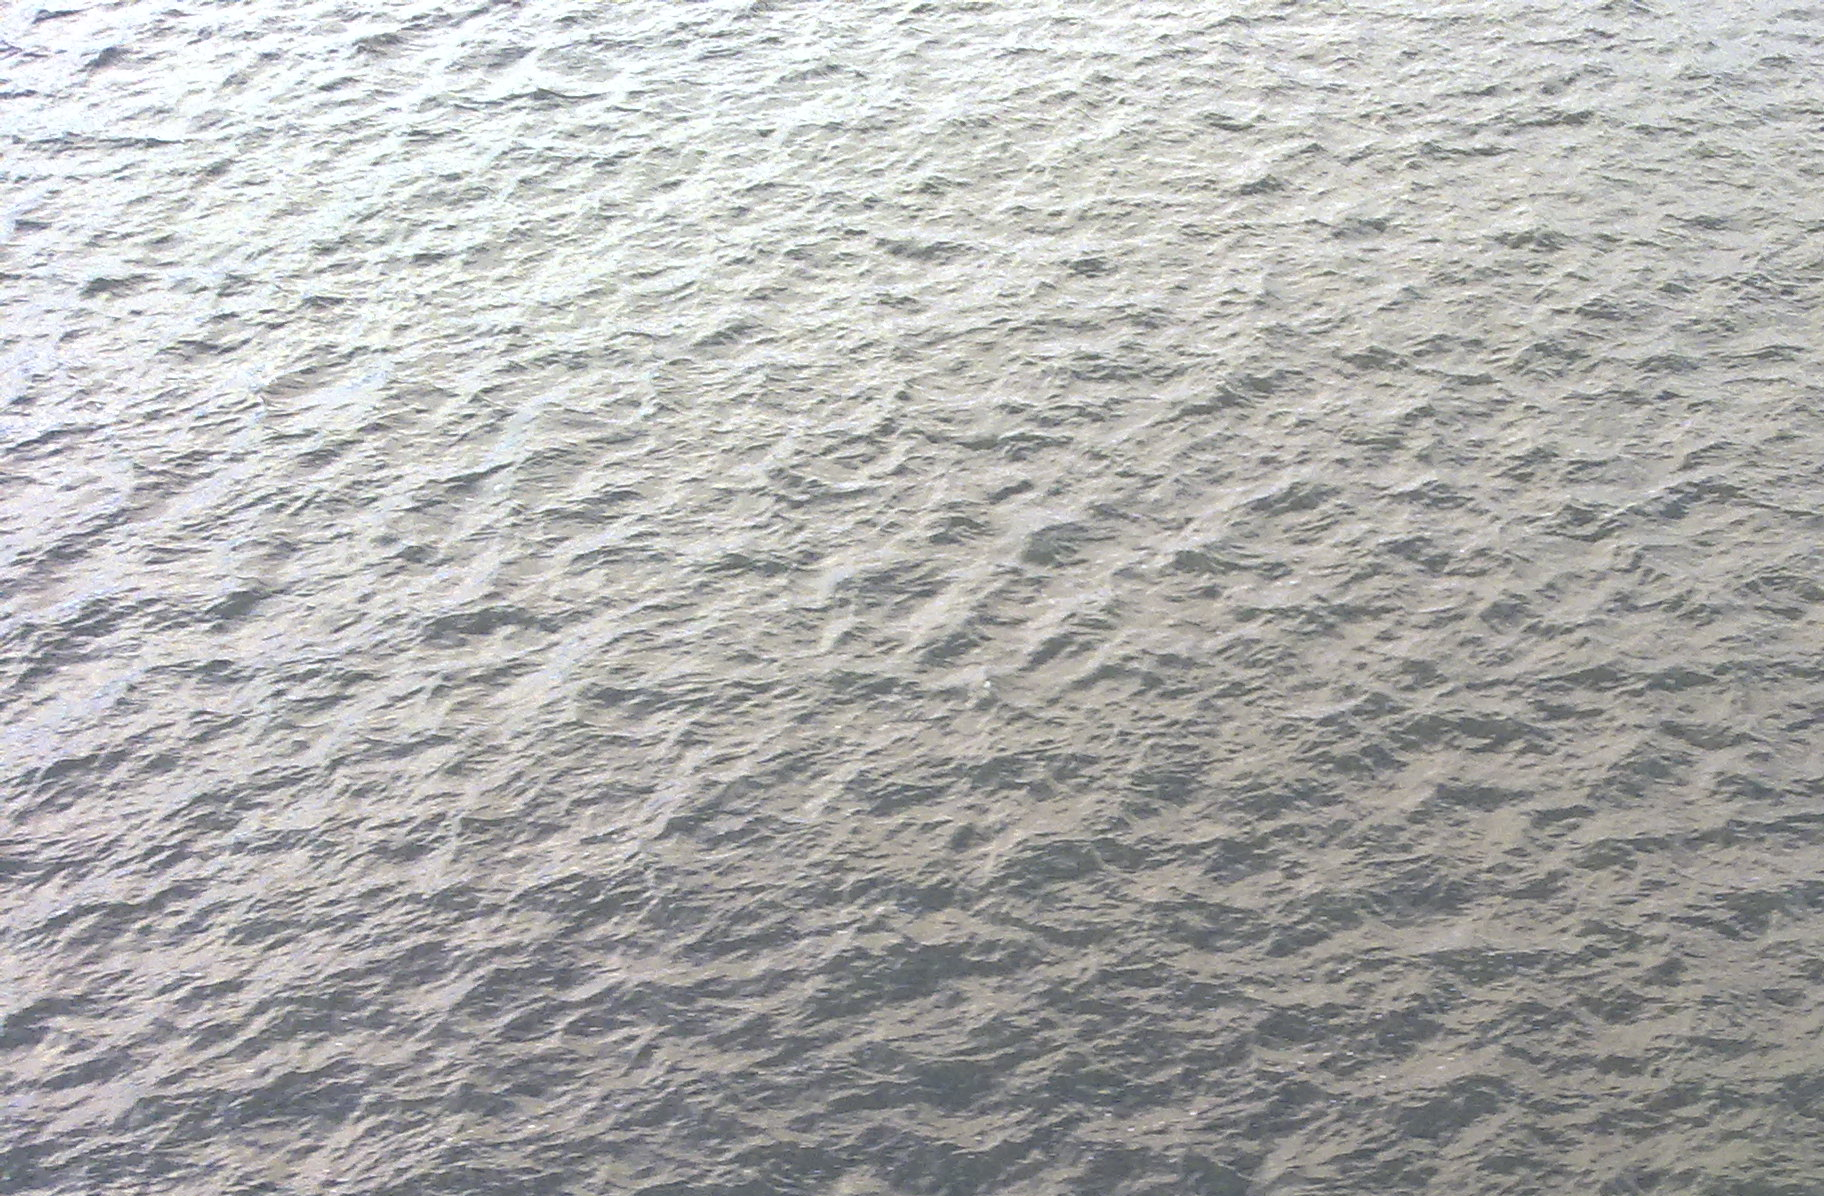
\includegraphics[width=.495\textwidth]{Images/Attribute/Baltic_Sea_from_ferry_small}}
    \subcaptionbox{\label{fig:sea_storm}}{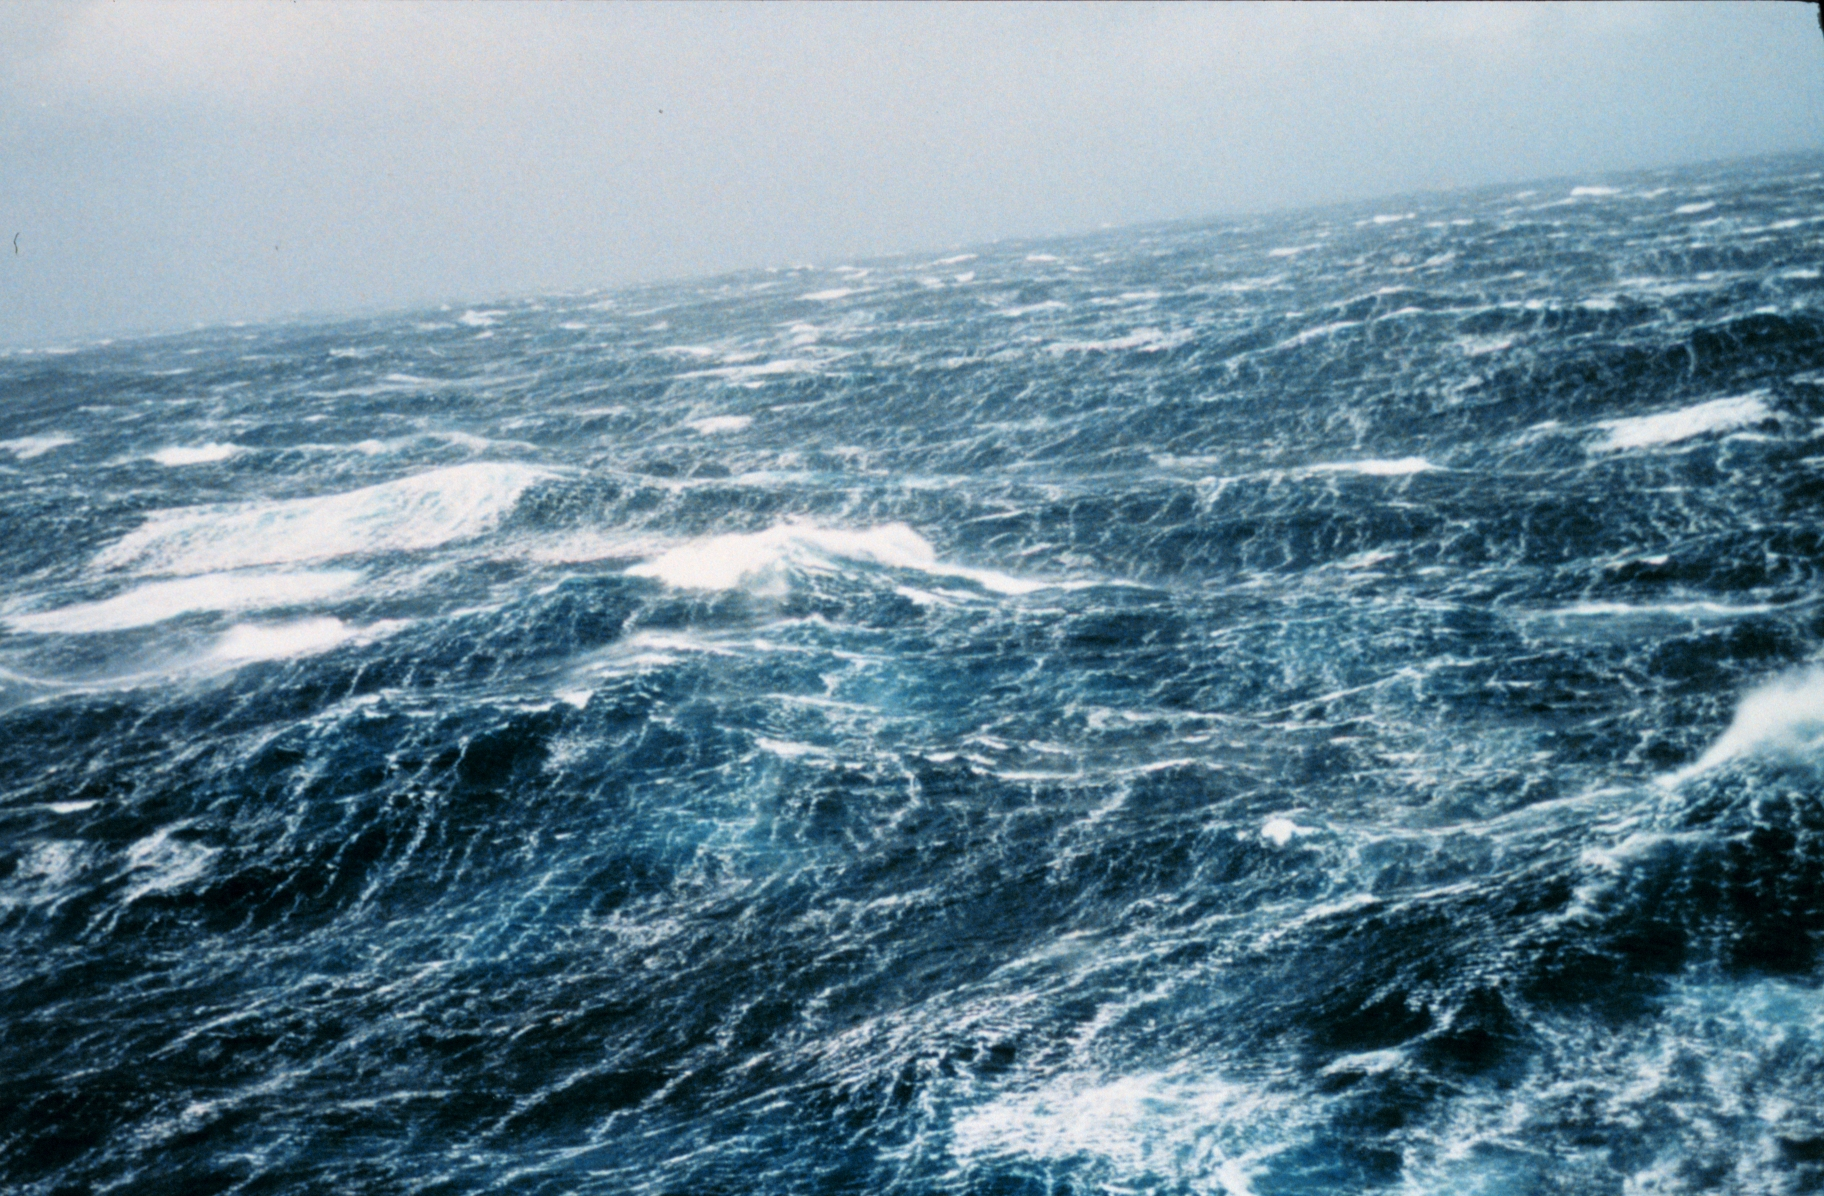
\includegraphics[width=0.495\textwidth]{Images/Public_domain/Wea00816}}
    \caption{Visual cues present on surfaces of large bodies of water include cues that make it possible to estimate the speed and direction of the wind, as well as cues that make it possible to estimate the distance to the surface. \subrefp{fig:small_waves} \idxse{low}{wind speed}{Low wind speeds} give rise to waves with \idxs{short}{wavelength} and no whitecaps. The frequency with wich the wave pattern changes is an importans visual cue when estimating the size of the waves which is necessary when estimating the distance to the surface. \subrefp{fig:small_waves} \idxse{high}{wind speed}{High wind speeds}, starting already at approximately 3.4~m/s, tend to break the crests of the waves and causes whitecaps. This phot was taken during a storm in the North Pacific Ocean the winter 1989.}
    \label{fig:sea_states}
\end{figure}

\subsection{Landing on ships with aircrafts}

A fighter aircraft that is about to land on an aircraft carrier has to approach the carrier from behind, and often slightly from the side. Therefore, the pilot has to know the orientation of the carrier. During landing, the carrier traveles with full speed against the wind in order to give the polit as high relative speed to the air as possible, creating a \wake behind itself, with a \backwash that is usually clearly visible for the pilot. The reason the backwash is usually seen so well is partly because it often contains a lot of \idxsp{air}{bubble}{s} that have been dragged down into the water or is covered by foam, and is therefore much brighter than the rest of the water, and partly because of the \turbulence that is created in the water as the ship passes by which makes the surface more blank. This backwash can be seen in \figref{fig:aircraft_carriers_and_backwash}.

In \figref{fig:aircraft_carrier_full_wake}, \idxsp{V-shaped}{wavefront}{s} after the ship can also be observed. These wavefronts form two \idxsp{wake}{line}{s}, one on each side of the backwash, which together are known as the \idxs{Kelvin}{wake pattern}\index{pattern!wake|see{Kelvin wake pattern}} after the British scientist \idxs{Lord}{Kelvin}.

\begin{figure}
    \centering
    \subcaptionbox{\label{fig:aircraft_carrier_full_wake}} {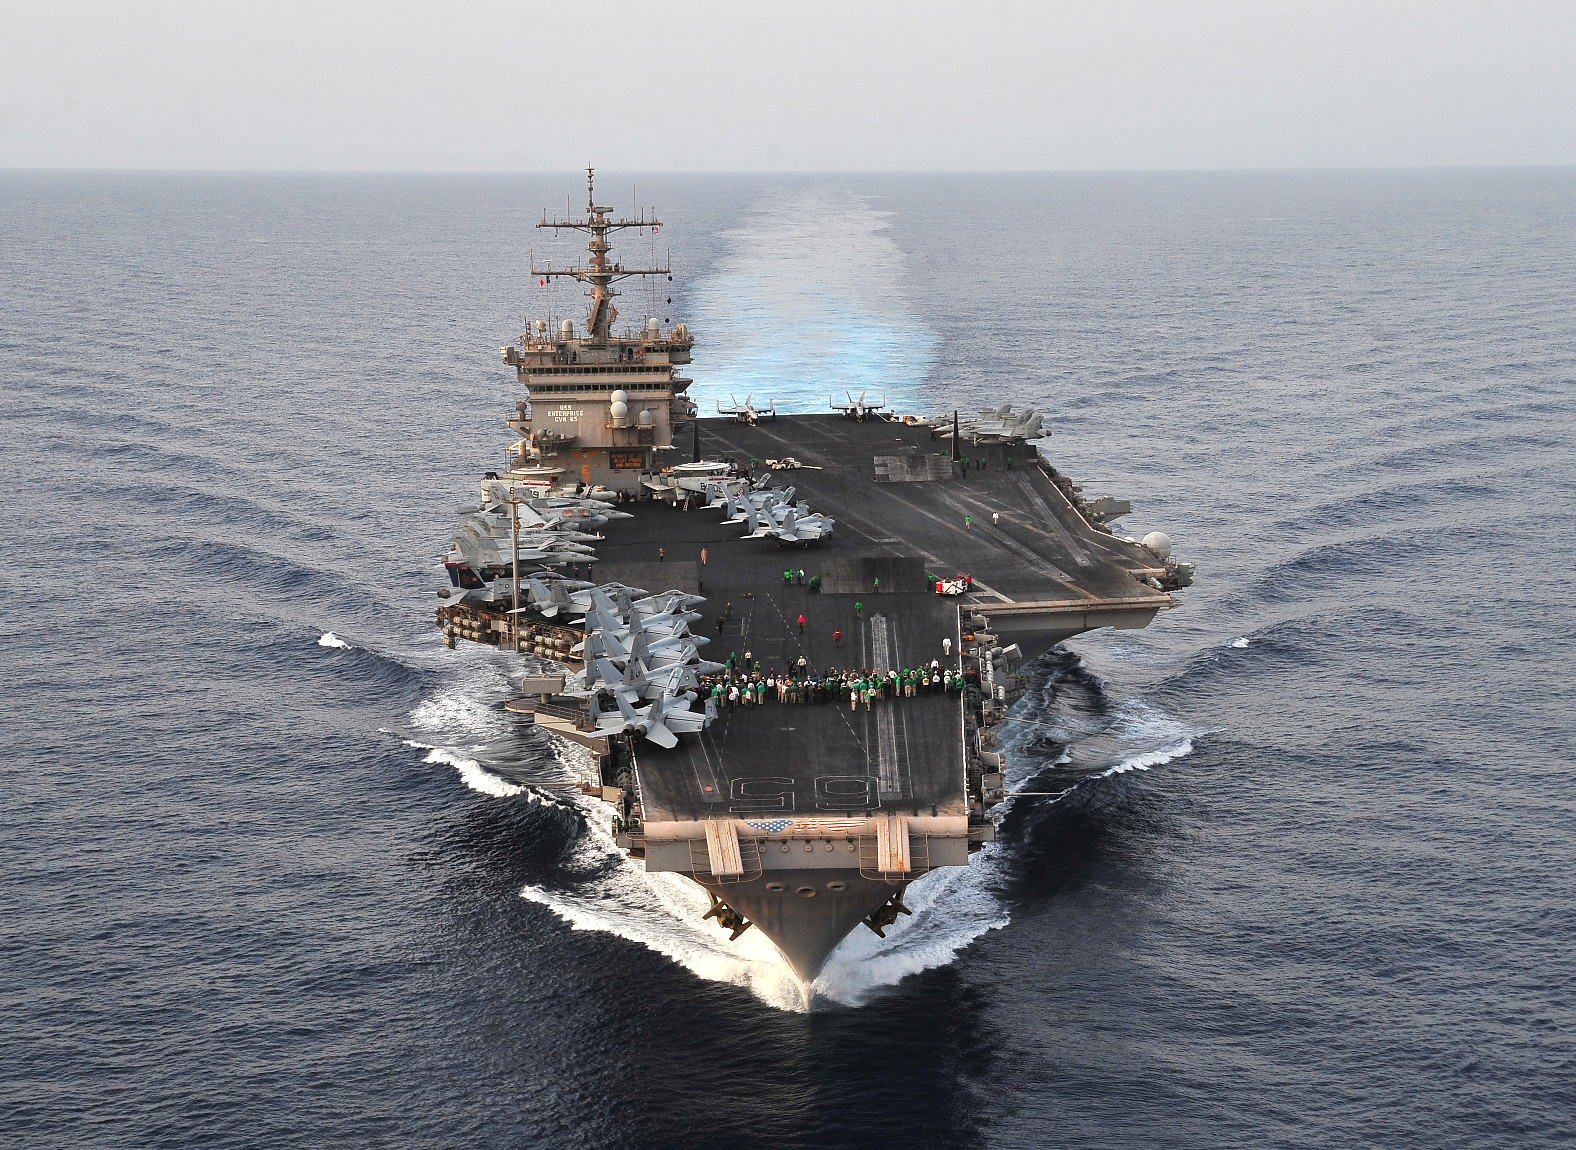
\includegraphics[width=0.495\textwidth]{Images/Public_domain/The_aircraft_carrier_USS_Enterprise_(CVN_65)}}
    \subcaptionbox{\label{fig:aircraft_carrier_landing_backwash}} {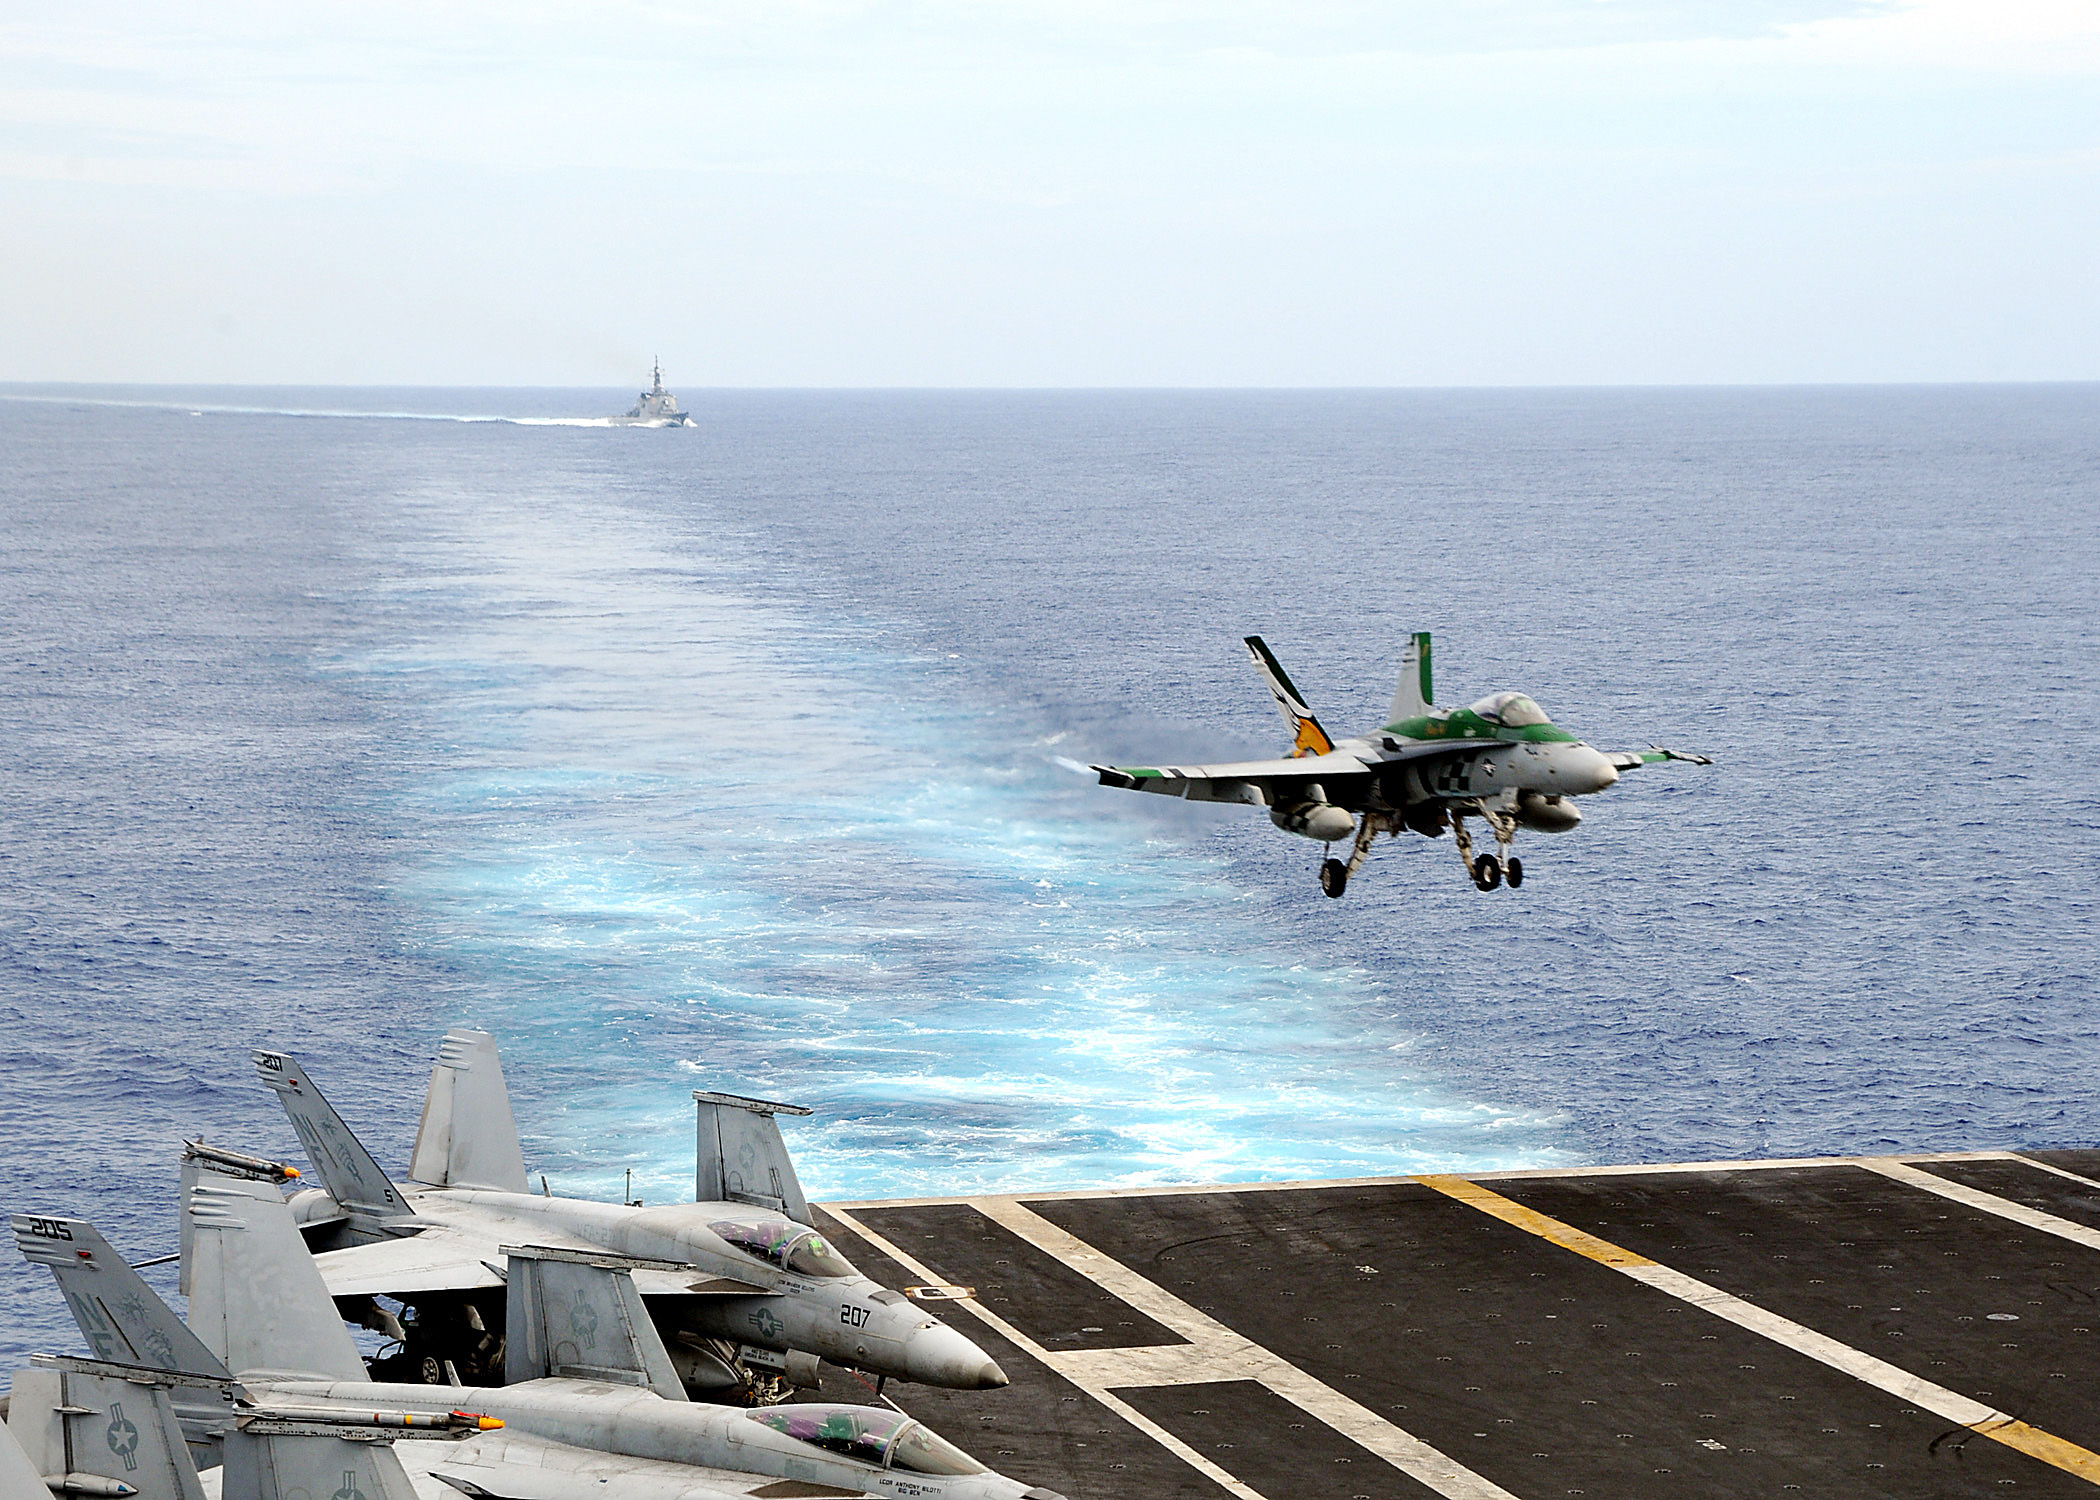
\includegraphics[width=0.495\textwidth]{Images/Public_domain/An_F-A-18C_Hornet_lands_on_the_aircraft_carrier_USS_George_Washington_(CVN_73)}}
    \caption{Aircraft carriers. Note the backwash created behind the ships, serving as a reference for aircraft pilots during landing. \subrefp{fig:aircraft_carrier_full_wake} The aircraft carrier USS Enterprise (CVN 65). \subrefp{fig:aircraft_carrier_landing_backwash} An F/A-18 Hornet landing on an aircraft carrier.}
    \label{fig:aircraft_carriers_and_backwash}
\end{figure}

In a real situationm, the pilot can look at the backwash and the wake lines created by the carrier in order to find the right angle with which to approach the carrier, as can be seen in \citep{Alivewithpassion2007,MatteoBram2007} (see also \figref{fig:aircraft_carrier_landing_backwash}). In a simulation, it is important that the pilot has the same possibility. It is therefore necessary that ships in the simulation leave a wake behind themselves that looks and behaves as a real wake, and that consists of both waves created by the ship and of a clearly visible backwash. It is valuable that this wake keeps alive and looks as a real wake for as long time as possible. As an example, this would make it possible for the pilot to determine the direction to a ship, even if the only thing that is spoted is a single \idxs{wake}{line}.